\section{CTCLTimer  Class Reference}
\label{classCTCLTimer}\index{CTCLTimer@{CTCLTimer}}
{\tt \#include $<$TCLTimer.h$>$}

Inheritance diagram for CTCLTimer::\begin{figure}[H]
\begin{center}
\leavevmode
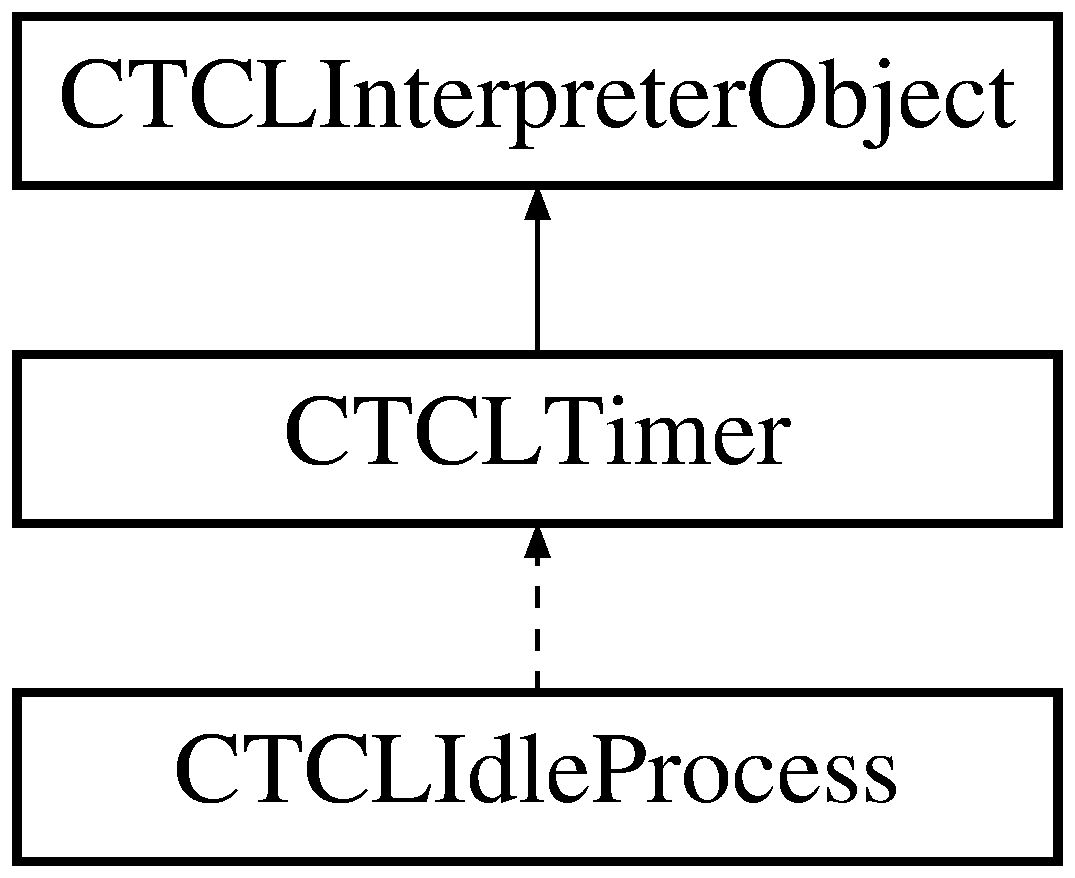
\includegraphics[height=3cm]{classCTCLTimer}
\end{center}
\end{figure}
\subsection*{Public Methods}
\begin{CompactItemize}
\item 
{\bf CTCLTimer} ()
\item 
{\bf CTCLTimer} ({\bf CTCLInterpreter} $\ast$p\-Interp, {\bf UInt\_\-t} n\-Msec=0)
\item 
virtual {\bf $\sim$CTCLTimer} ()
\item 
Tk\_\-Timer\-Token {\bf get\-Token} () const
\item 
{\bf UInt\_\-t} {\bf get\-Msec} () const
\item 
{\bf Bool\_\-t} {\bf Is\-Set} () const
\item 
virtual void {\bf operator()} ()=0
\item 
void {\bf Set} ()
\item 
void {\bf Set} ({\bf UInt\_\-t} nms)
\item 
void {\bf Clear} ()
\end{CompactItemize}
\subsection*{Static Public Methods}
\begin{CompactItemize}
\item 
void {\bf Callback\-Relay} (Client\-Data p\-Object)
\end{CompactItemize}
\subsection*{Protected Methods}
\begin{CompactItemize}
\item 
void {\bf set\-Token} (Tk\_\-Timer\-Token am\_\-t\-Token)
\item 
void {\bf set\-Msec} ({\bf UInt\_\-t} am\_\-n\-Msec)
\item 
void {\bf set\-Set} ({\bf Bool\_\-t} am\_\-f\-Set)
\end{CompactItemize}
\subsection*{Private Methods}
\begin{CompactItemize}
\item 
{\bf CTCLTimer} (const CTCLTimer \&a\-CTCLTimer)
\item 
CTCLTimer \& {\bf operator=} (const CTCLTimer \&a\-CTCLTimer)
\item 
int {\bf operator==} (const CTCLTimer \&a\-CTCLTimer)
\end{CompactItemize}
\subsection*{Private Attributes}
\begin{CompactItemize}
\item 
Tk\_\-Timer\-Token {\bf m\_\-t\-Token}
\item 
{\bf UInt\_\-t} {\bf m\_\-n\-Msec}
\item 
{\bf Bool\_\-t} {\bf m\_\-f\-Set}
\end{CompactItemize}


\subsection{Constructor \& Destructor Documentation}
\index{CTCLTimer@{CTCLTimer}!CTCLTimer@{CTCLTimer}}
\index{CTCLTimer@{CTCLTimer}!CTCLTimer@{CTCLTimer}}
\subsubsection{\setlength{\rightskip}{0pt plus 5cm}CTCLTimer::CTCLTimer ()\hspace{0.3cm}{\tt  [inline]}}\label{classCTCLTimer_a0}




Definition at line 324 of file TCLTimer.h.

References m\_\-f\-Set, m\_\-n\-Msec, and m\_\-t\-Token.\index{CTCLTimer@{CTCLTimer}!CTCLTimer@{CTCLTimer}}
\index{CTCLTimer@{CTCLTimer}!CTCLTimer@{CTCLTimer}}
\subsubsection{\setlength{\rightskip}{0pt plus 5cm}CTCLTimer::CTCLTimer ({\bf CTCLInterpreter} $\ast$ {\em p\-Interp}, {\bf UInt\_\-t} {\em n\-Msec} = 0)\hspace{0.3cm}{\tt  [inline]}}\label{classCTCLTimer_a1}




Definition at line 330 of file TCLTimer.h.

References m\_\-f\-Set, m\_\-n\-Msec, m\_\-t\-Token, and UInt\_\-t.\index{CTCLTimer@{CTCLTimer}!~CTCLTimer@{$\sim$CTCLTimer}}
\index{~CTCLTimer@{$\sim$CTCLTimer}!CTCLTimer@{CTCLTimer}}
\subsubsection{\setlength{\rightskip}{0pt plus 5cm}virtual CTCLTimer::$\sim$CTCLTimer ()\hspace{0.3cm}{\tt  [inline, virtual]}}\label{classCTCLTimer_a2}




Definition at line 336 of file TCLTimer.h.

References Clear().\index{CTCLTimer@{CTCLTimer}!CTCLTimer@{CTCLTimer}}
\index{CTCLTimer@{CTCLTimer}!CTCLTimer@{CTCLTimer}}
\subsubsection{\setlength{\rightskip}{0pt plus 5cm}CTCLTimer::CTCLTimer (const CTCLTimer \& {\em a\-CTCLTimer})\hspace{0.3cm}{\tt  [private]}}\label{classCTCLTimer_c0}




\subsection{Member Function Documentation}
\index{CTCLTimer@{CTCLTimer}!CallbackRelay@{CallbackRelay}}
\index{CallbackRelay@{CallbackRelay}!CTCLTimer@{CTCLTimer}}
\subsubsection{\setlength{\rightskip}{0pt plus 5cm}void CTCLTimer::Callback\-Relay (Client\-Data {\em p\-Object})\hspace{0.3cm}{\tt  [static]}}\label{classCTCLTimer_d0}




Definition at line 321 of file TCLTimer.cpp.

References m\_\-f\-Set.

Referenced by Set().\index{CTCLTimer@{CTCLTimer}!Clear@{Clear}}
\index{Clear@{Clear}!CTCLTimer@{CTCLTimer}}
\subsubsection{\setlength{\rightskip}{0pt plus 5cm}void CTCLTimer::Clear ()}\label{classCTCLTimer_a9}




Reimplemented in {\bf CTCLIdle\-Process} {\rm (p.\,\pageref{classCTCLIdleProcess_a5})}.

Definition at line 369 of file TCLTimer.cpp.

References m\_\-f\-Set, and m\_\-t\-Token.

Referenced by CTCLIdle\-Process::Clear(), and $\sim$CTCLTimer().\index{CTCLTimer@{CTCLTimer}!getMsec@{getMsec}}
\index{getMsec@{getMsec}!CTCLTimer@{CTCLTimer}}
\subsubsection{\setlength{\rightskip}{0pt plus 5cm}{\bf UInt\_\-t} CTCLTimer::get\-Msec () const\hspace{0.3cm}{\tt  [inline]}}\label{classCTCLTimer_a4}




Definition at line 360 of file TCLTimer.h.

References m\_\-n\-Msec, and UInt\_\-t.\index{CTCLTimer@{CTCLTimer}!getToken@{getToken}}
\index{getToken@{getToken}!CTCLTimer@{CTCLTimer}}
\subsubsection{\setlength{\rightskip}{0pt plus 5cm}Tk\_\-Timer\-Token CTCLTimer::get\-Token () const\hspace{0.3cm}{\tt  [inline]}}\label{classCTCLTimer_a3}




Definition at line 356 of file TCLTimer.h.

References m\_\-t\-Token.\index{CTCLTimer@{CTCLTimer}!IsSet@{IsSet}}
\index{IsSet@{IsSet}!CTCLTimer@{CTCLTimer}}
\subsubsection{\setlength{\rightskip}{0pt plus 5cm}{\bf Bool\_\-t} CTCLTimer::Is\-Set () const\hspace{0.3cm}{\tt  [inline]}}\label{classCTCLTimer_a5}




Definition at line 364 of file TCLTimer.h.

References Bool\_\-t, and m\_\-f\-Set.\index{CTCLTimer@{CTCLTimer}!operator()@{operator()}}
\index{operator()@{operator()}!CTCLTimer@{CTCLTimer}}
\subsubsection{\setlength{\rightskip}{0pt plus 5cm}virtual void CTCLTimer::operator() ()\hspace{0.3cm}{\tt  [pure virtual]}}\label{classCTCLTimer_a6}




Implemented in {\bf CTCLIdle\-Process} {\rm (p.\,\pageref{classCTCLIdleProcess_a6})}.\index{CTCLTimer@{CTCLTimer}!operator=@{operator=}}
\index{operator=@{operator=}!CTCLTimer@{CTCLTimer}}
\subsubsection{\setlength{\rightskip}{0pt plus 5cm}CTCLTimer\& CTCLTimer::operator= (const CTCLTimer \& {\em a\-CTCLTimer})\hspace{0.3cm}{\tt  [private]}}\label{classCTCLTimer_c1}


\index{CTCLTimer@{CTCLTimer}!operator==@{operator==}}
\index{operator==@{operator==}!CTCLTimer@{CTCLTimer}}
\subsubsection{\setlength{\rightskip}{0pt plus 5cm}int CTCLTimer::operator== (const CTCLTimer \& {\em a\-CTCLTimer})\hspace{0.3cm}{\tt  [private]}}\label{classCTCLTimer_c2}


\index{CTCLTimer@{CTCLTimer}!Set@{Set}}
\index{Set@{Set}!CTCLTimer@{CTCLTimer}}
\subsubsection{\setlength{\rightskip}{0pt plus 5cm}void CTCLTimer::Set ({\bf UInt\_\-t} {\em nms})\hspace{0.3cm}{\tt  [inline]}}\label{classCTCLTimer_a8}




Definition at line 390 of file TCLTimer.h.

References m\_\-n\-Msec, Set(), and UInt\_\-t.\index{CTCLTimer@{CTCLTimer}!Set@{Set}}
\index{Set@{Set}!CTCLTimer@{CTCLTimer}}
\subsubsection{\setlength{\rightskip}{0pt plus 5cm}void CTCLTimer::Set ()}\label{classCTCLTimer_a7}




Reimplemented in {\bf CTCLIdle\-Process} {\rm (p.\,\pageref{classCTCLIdleProcess_a4})}.

Definition at line 344 of file TCLTimer.cpp.

References Callback\-Relay(), m\_\-f\-Set, m\_\-n\-Msec, and m\_\-t\-Token.

Referenced by Set(), and CTCLIdle\-Process::Set().\index{CTCLTimer@{CTCLTimer}!setMsec@{setMsec}}
\index{setMsec@{setMsec}!CTCLTimer@{CTCLTimer}}
\subsubsection{\setlength{\rightskip}{0pt plus 5cm}void CTCLTimer::set\-Msec ({\bf UInt\_\-t} {\em am\_\-n\-Msec})\hspace{0.3cm}{\tt  [inline, protected]}}\label{classCTCLTimer_b1}




Definition at line 376 of file TCLTimer.h.

References m\_\-n\-Msec, and UInt\_\-t.\index{CTCLTimer@{CTCLTimer}!setSet@{setSet}}
\index{setSet@{setSet}!CTCLTimer@{CTCLTimer}}
\subsubsection{\setlength{\rightskip}{0pt plus 5cm}void CTCLTimer::set\-Set ({\bf Bool\_\-t} {\em am\_\-f\-Set})\hspace{0.3cm}{\tt  [inline, protected]}}\label{classCTCLTimer_b2}




Definition at line 380 of file TCLTimer.h.

References Bool\_\-t, and m\_\-f\-Set.\index{CTCLTimer@{CTCLTimer}!setToken@{setToken}}
\index{setToken@{setToken}!CTCLTimer@{CTCLTimer}}
\subsubsection{\setlength{\rightskip}{0pt plus 5cm}void CTCLTimer::set\-Token (Tk\_\-Timer\-Token {\em am\_\-t\-Token})\hspace{0.3cm}{\tt  [inline, protected]}}\label{classCTCLTimer_b0}




Definition at line 372 of file TCLTimer.h.

References m\_\-t\-Token.

\subsection{Member Data Documentation}
\index{CTCLTimer@{CTCLTimer}!m_fSet@{m\_\-fSet}}
\index{m_fSet@{m\_\-fSet}!CTCLTimer@{CTCLTimer}}
\subsubsection{\setlength{\rightskip}{0pt plus 5cm}{\bf Bool\_\-t} CTCLTimer::m\_\-f\-Set\hspace{0.3cm}{\tt  [private]}}\label{classCTCLTimer_o2}




Definition at line 319 of file TCLTimer.h.

Referenced by Callback\-Relay(), Clear(), CTCLTimer(), Is\-Set(), Set(), and set\-Set().\index{CTCLTimer@{CTCLTimer}!m_nMsec@{m\_\-nMsec}}
\index{m_nMsec@{m\_\-nMsec}!CTCLTimer@{CTCLTimer}}
\subsubsection{\setlength{\rightskip}{0pt plus 5cm}{\bf UInt\_\-t} CTCLTimer::m\_\-n\-Msec\hspace{0.3cm}{\tt  [private]}}\label{classCTCLTimer_o1}




Definition at line 318 of file TCLTimer.h.

Referenced by CTCLTimer(), get\-Msec(), Set(), and set\-Msec().\index{CTCLTimer@{CTCLTimer}!m_tToken@{m\_\-tToken}}
\index{m_tToken@{m\_\-tToken}!CTCLTimer@{CTCLTimer}}
\subsubsection{\setlength{\rightskip}{0pt plus 5cm}Tk\_\-Timer\-Token CTCLTimer::m\_\-t\-Token\hspace{0.3cm}{\tt  [private]}}\label{classCTCLTimer_o0}




Definition at line 317 of file TCLTimer.h.

Referenced by Clear(), CTCLTimer(), get\-Token(), Set(), and set\-Token().

The documentation for this class was generated from the following files:\begin{CompactItemize}
\item 
{\bf TCLTimer.h}\item 
{\bf TCLTimer.cpp}\end{CompactItemize}
